\documentclass{standalone}
\usepackage{tikz}
\usetikzlibrary{patterns, positioning}
\usepackage[sfdefault]{ClearSans} %% option 'sfdefault' activates Clear Sans as the default text font
\usepackage[T1]{fontenc}

\begin{document}
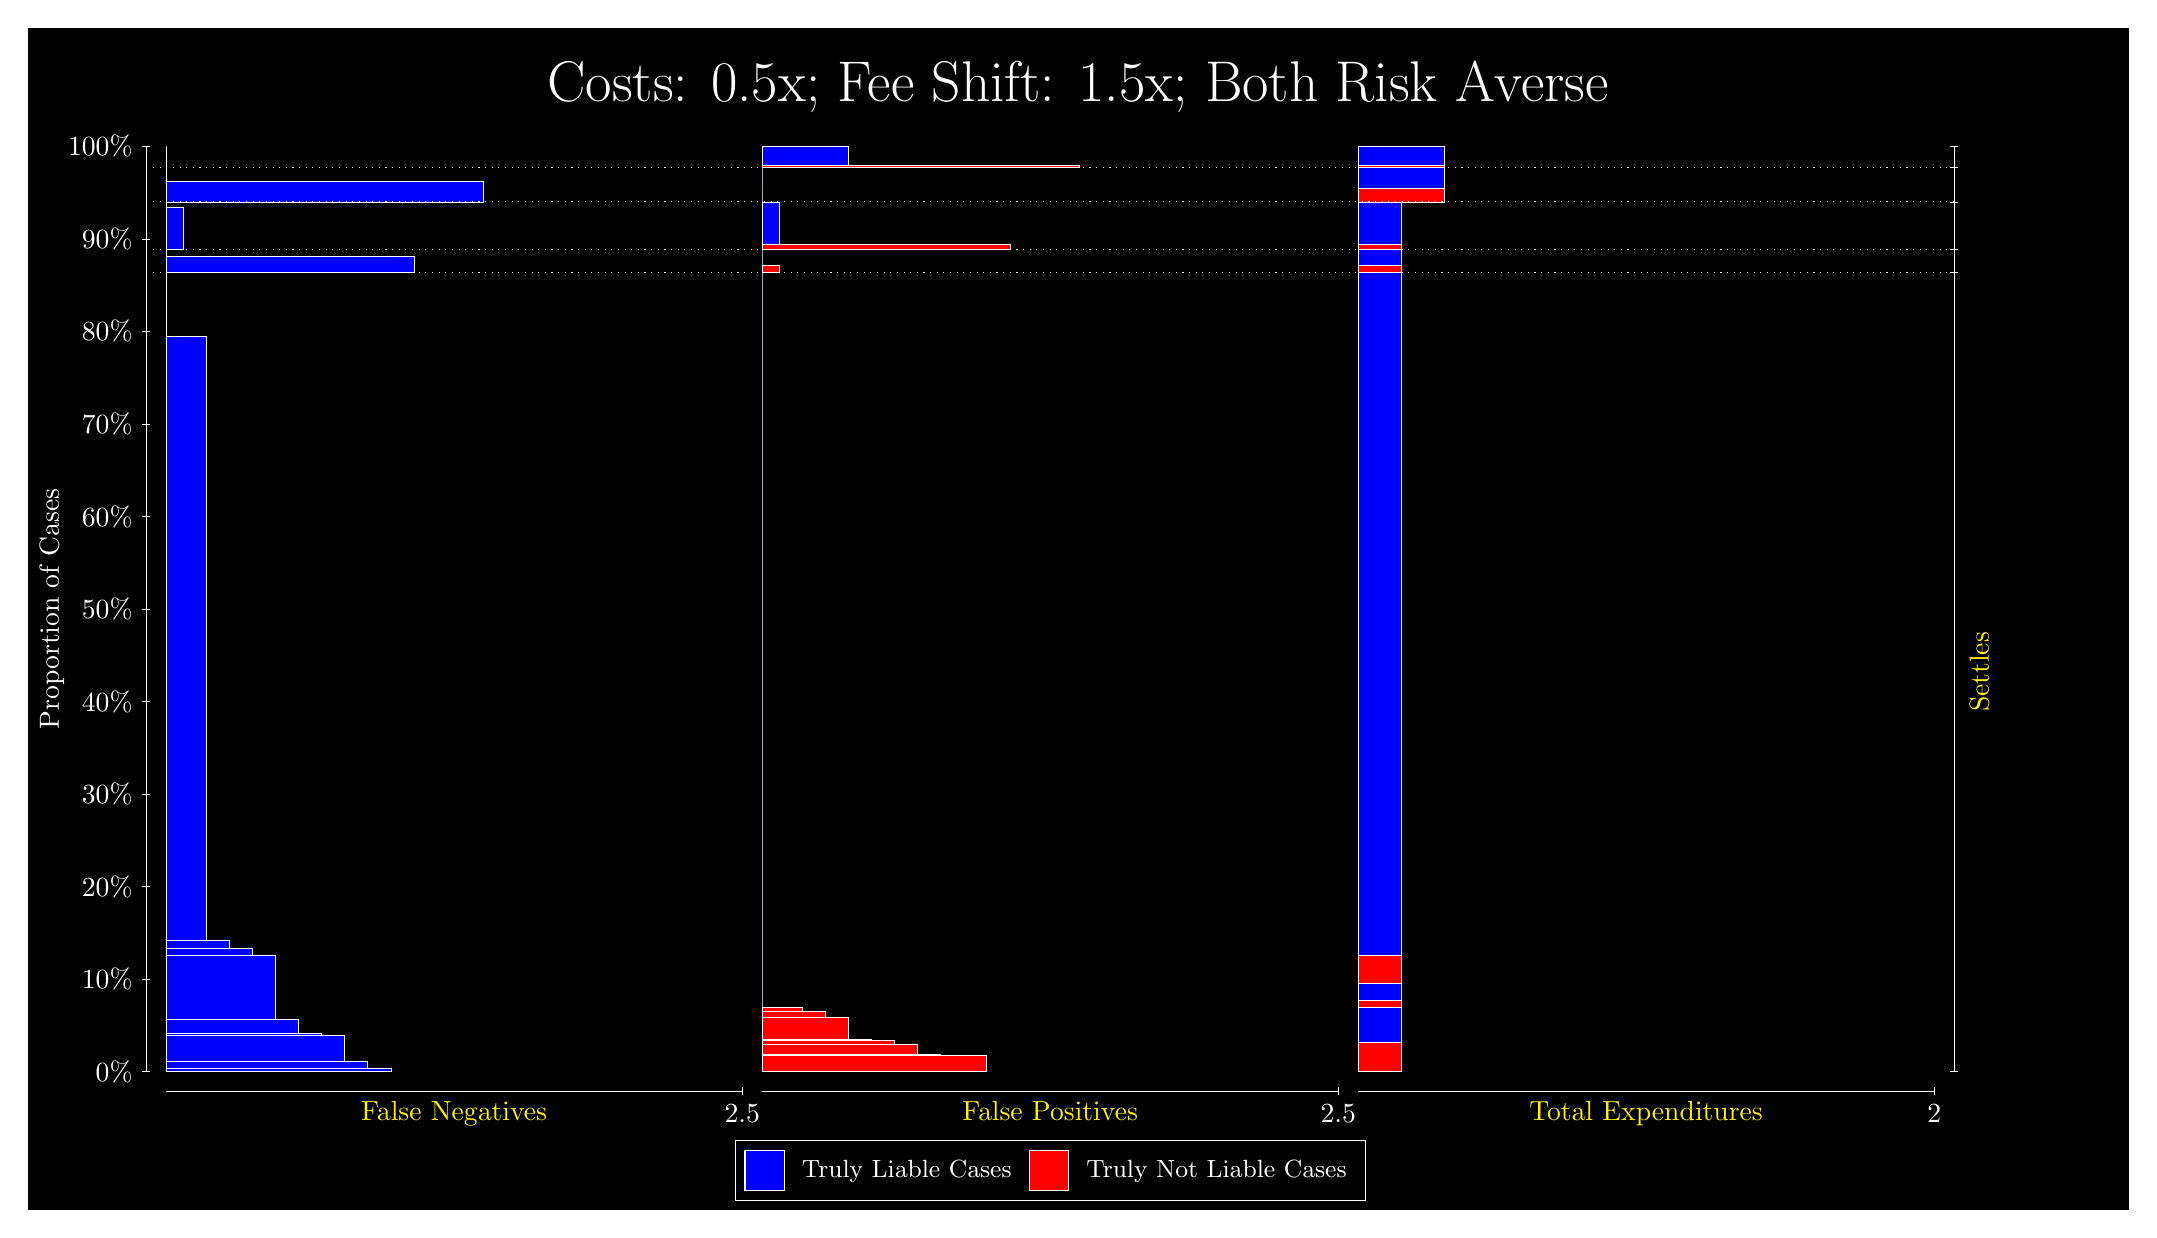
\begin{tikzpicture}
\draw[fill=black] (0,0) rectangle (26.667,15);
\draw[text=white] (0,13.5) rectangle (26.667,15) node[midway] {\huge Costs: 0.5x; Fee Shift: 1.5x; Both Risk Averse};
\draw[white, very thin] (1.5,1.75) -- (1.5,13.5);
\node[rotate=90, text=white, anchor=center] at (0.3, 7.625) {Proportion of Cases};
\draw[white, very thin] (1.45,1.75) -- (1.55,1.75);
\node[text=white, anchor=east] at (1.45, 1.75) {0\%};
\draw[white, very thin] (1.45,2.925) -- (1.55,2.925);
\node[text=white, anchor=east] at (1.45, 2.925) {10\%};
\draw[white, very thin] (1.45,4.1) -- (1.55,4.1);
\node[text=white, anchor=east] at (1.45, 4.1) {20\%};
\draw[white, very thin] (1.45,5.275) -- (1.55,5.275);
\node[text=white, anchor=east] at (1.45, 5.275) {30\%};
\draw[white, very thin] (1.45,6.45) -- (1.55,6.45);
\node[text=white, anchor=east] at (1.45, 6.45) {40\%};
\draw[white, very thin] (1.45,7.625) -- (1.55,7.625);
\node[text=white, anchor=east] at (1.45, 7.625) {50\%};
\draw[white, very thin] (1.45,8.8) -- (1.55,8.8);
\node[text=white, anchor=east] at (1.45, 8.8) {60\%};
\draw[white, very thin] (1.45,9.975) -- (1.55,9.975);
\node[text=white, anchor=east] at (1.45, 9.975) {70\%};
\draw[white, very thin] (1.45,11.15) -- (1.55,11.15);
\node[text=white, anchor=east] at (1.45, 11.15) {80\%};
\draw[white, very thin] (1.45,12.325) -- (1.55,12.325);
\node[text=white, anchor=east] at (1.45, 12.325) {90\%};
\draw[white, very thin] (1.45,13.5) -- (1.55,13.5);
\node[text=white, anchor=east] at (1.45, 13.5) {100\%};

\draw[white, very thin] (24.457,1.75) -- (24.457,13.5);
\draw[white, very thin] (24.407,1.75) -- (24.507,1.75);
\node[anchor=west] at (24.407, 1.75) {};
\draw[white, very thin] (24.407,11.901) -- (24.507,11.901);
\node[anchor=west] at (24.407, 11.901) {};
\draw[white, very thin] (24.407,12.19) -- (24.507,12.19);
\node[anchor=west] at (24.407, 12.19) {};
\draw[white, very thin] (24.407,12.795) -- (24.507,12.795);
\node[anchor=west] at (24.407, 12.795) {};
\draw[white, very thin] (24.407,13.233) -- (24.507,13.233);
\node[anchor=west] at (24.407, 13.233) {};
\draw[white, very thin] (24.407,13.5) -- (24.507,13.5);
\node[anchor=west] at (24.407, 13.5) {};

\draw[white, very thin, fill=blue] (1.75,1.75) rectangle (4.6044,1.7903);
\draw[white, very thin, fill=blue] (1.75,1.7903) rectangle (4.3116,1.875);
\draw[white, very thin, fill=blue] (1.75,1.875) rectangle (4.0188,2.2068);
\draw[white, very thin, fill=blue] (1.75,2.2068) rectangle (3.7261,2.2339);
\draw[white, very thin, fill=blue] (1.75,2.2339) rectangle (3.4333,2.4125);
\draw[white, very thin, fill=blue] (1.75,2.4125) rectangle (3.1406,3.2203);
\draw[white, very thin, fill=blue] (1.75,3.2203) rectangle (2.8478,3.3168);
\draw[white, very thin, fill=blue] (1.75,3.3168) rectangle (2.5551,3.4131);
\draw[white, very thin, fill=blue] (1.75,3.4131) rectangle (2.2623,11.091);
\draw[white, very thin, fill=red] (1.75,11.091) rectangle (1.75,11.901);
\draw[white, very thin, fill=blue] (1.75,11.901) rectangle (4.8971,12.098);
\draw[white, very thin, fill=red] (1.75,12.098) rectangle (1.75,12.19);
\draw[white, very thin, fill=blue] (1.75,12.19) rectangle (1.9696,12.723);
\draw[white, very thin, fill=red] (1.75,12.723) rectangle (1.75,12.795);
\draw[white, very thin, fill=blue] (1.75,12.795) rectangle (5.7754,13.06);
\draw[white, very thin, fill=red] (1.75,13.06) rectangle (1.75,13.233);
\draw[white, very thin, fill=red] (1.75,13.233) rectangle (1.75,13.261);
\draw[white, very thin, fill=blue] (1.75,13.261) rectangle (1.75,13.5);
\draw[white, very thin, fill=red] (9.3189,1.75) rectangle (12.173,1.951);
\draw[white, very thin, fill=red] (9.3189,1.951) rectangle (11.88,1.9622);
\draw[white, very thin, fill=red] (9.3189,1.9622) rectangle (11.588,1.974);
\draw[white, very thin, fill=red] (9.3189,1.974) rectangle (11.295,2.1016);
\draw[white, very thin, fill=red] (9.3189,2.1016) rectangle (11.002,2.1487);
\draw[white, very thin, fill=red] (9.3189,2.1487) rectangle (10.709,2.1607);
\draw[white, very thin, fill=red] (9.3189,2.1607) rectangle (10.709,2.1645);
\draw[white, very thin, fill=red] (9.3189,2.1645) rectangle (10.417,2.4354);
\draw[white, very thin, fill=red] (9.3189,2.4354) rectangle (10.124,2.521);
\draw[white, very thin, fill=red] (9.3189,2.521) rectangle (9.8312,2.56);
\draw[white, very thin, fill=blue] (9.3189,2.56) rectangle (9.3189,11.901);
\draw[white, very thin, fill=red] (9.3189,11.901) rectangle (9.5384,11.993);
\draw[white, very thin, fill=blue] (9.3189,11.993) rectangle (9.3189,12.19);
\draw[white, very thin, fill=red] (9.3189,12.19) rectangle (12.466,12.262);
\draw[white, very thin, fill=blue] (9.3189,12.262) rectangle (9.5384,12.795);
\draw[white, very thin, fill=red] (9.3189,12.795) rectangle (9.3189,12.967);
\draw[white, very thin, fill=blue] (9.3189,12.967) rectangle (9.3189,13.233);
\draw[white, very thin, fill=red] (9.3189,13.233) rectangle (13.344,13.261);
\draw[white, very thin, fill=blue] (9.3189,13.261) rectangle (10.417,13.5);
\draw[white, very thin, fill=red] (16.888,1.75) rectangle (17.437,2.1223);
\draw[white, very thin, fill=blue] (16.888,2.1223) rectangle (17.437,2.5659);
\draw[white, very thin, fill=red] (16.888,2.5659) rectangle (17.437,2.652);
\draw[white, very thin, fill=blue] (16.888,2.652) rectangle (17.437,2.8709);
\draw[white, very thin, fill=red] (16.888,2.8709) rectangle (17.437,3.2225);
\draw[white, very thin, fill=blue] (16.888,3.2225) rectangle (17.437,11.901);
\draw[white, very thin, fill=red] (16.888,11.901) rectangle (17.437,11.993);
\draw[white, very thin, fill=blue] (16.888,11.993) rectangle (17.437,12.19);
\draw[white, very thin, fill=red] (16.888,12.19) rectangle (17.437,12.262);
\draw[white, very thin, fill=blue] (16.888,12.262) rectangle (17.437,12.795);
\draw[white, very thin, fill=red] (16.888,12.795) rectangle (17.986,12.967);
\draw[white, very thin, fill=blue] (16.888,12.967) rectangle (17.986,13.233);
\draw[white, very thin, fill=red] (16.888,13.233) rectangle (17.986,13.261);
\draw[white, very thin, fill=blue] (16.888,13.261) rectangle (17.986,13.5);
\draw[white, dotted] (1.5,11.901) -- (24.457,11.901);
\draw[white, dotted] (1.5,12.19) -- (24.457,12.19);
\draw[white, dotted] (1.5,12.795) -- (24.457,12.795);
\draw[white, dotted] (1.5,13.233) -- (24.457,13.233);
\draw[white, very thin] (1.75,1.5) -- (9.0689,1.5);
\node[text=yellow, anchor=north] at (5.4094, 1.5) {False Negatives};
\draw[white, very thin] (9.0689,1.45) -- (9.0689,1.55);
\node[text=white, anchor=north] at (9.0689, 1.45) {2.5};

\draw[white, very thin] (9.3189,1.5) -- (16.638,1.5);
\node[text=yellow, anchor=north] at (12.978, 1.5) {False Positives};
\draw[white, very thin] (16.638,1.45) -- (16.638,1.55);
\node[text=white, anchor=north] at (16.638, 1.45) {2.5};

\draw[white, very thin] (16.888,1.5) -- (24.207,1.5);
\node[text=yellow, anchor=north] at (20.547, 1.5) {Total Expenditures};
\draw[white, very thin] (24.207,1.45) -- (24.207,1.55);
\node[text=white, anchor=north] at (24.207, 1.45) {2};

\node[text=yellow, centered, rotate=90] at (24.777, 6.8256) {Settles};





\draw (12.978300999999998,1.5) node[draw=none] (baseCoordinate) {};
\begin{scope}[align=center]
        \matrix[scale=0.5, draw=white, below=0.5cm of baseCoordinate, nodes={draw}, column sep=0.1cm]{
            \node[rectangle, draw, minimum width=0.5cm, minimum height=0.5cm, fill=blue] {}; &
            \node[draw=none, font=\small, text=white] (B) {Truly Liable Cases}; &
            \node[rectangle, draw, minimum width=0.5cm, minimum height=0.5cm, fill=red] {}; &
            \node[draw=none, font=\small, text=white] (B) {Truly Not Liable Cases}; \\
            };
\end{scope}

\end{tikzpicture}
\end{document}